\section{Improved Encoding}

HTTP/1.1 is a text\hyp{}based protocol, which means that all the request and response metadata uses a specific encoding called ASCII\@. This metadata\footnote{Known as the `headers', as opposed to the actual data being transferred which is known as the `body'.} includes things such as the content length (how much data is about to be transmitted), the content type (whether the data is text, audio, video etc.), which type of device the request originated from (including OS and browser), and authentication data. In ASCII, each byte (8 `bits' -- can also be thought of as a number between 0 and 255 inclusive) represents a single character of text (such as a letter or punctuation mark). For example the word `HTTP' is encoded as the sequence of bytes 72, 84, 84, 80.

Additionally, any numbers that need to be sent (such as the content length) are also represented digit by digit: `1234' would be represented as 49, 50, 51, 52. Considering that each individual byte can have 256 discrete possible values, this is quite wasteful, since it means that a four\hyp{}byte sequence can have $ (2^8)^4 = 2^{32} = 4294967296 $ possible values. All the numbers between zero and 1234 (inclusive) can be stored in $ \lceil \log_{2} 1235 \rceil = 11 $ bits, which is around a third of the length that it would be in the ASCII encoding.

As well as being very wasteful, text\hyp{}based protocols in general suffer from issues surrounding handling of whitespace (which just refers to spaces, `new line' or `tab' characters) and capitalisation. Overall, text-based protocols are both wasteful in terms of bandwidth and are often slower for a computer program to parse~\cite{http2faqbinary}. The major benefit of using text protocols is that they are easier for humans to read which in turn makes them easier to debug, but in practice this is rarely useful (due to tools which can format the data for you).

Therefore HTTP/2 adopts a binary protocol (that is to say one that is merely not textual), and additionally adopts a header compression scheme known as HPACK~\cite{hpack}~\footnote{HTTP/1.1 previously specified a method for compressing the \textit{body} of requests and responses, which is retained in HTTP/2, but previously there was no mechanism for compressing the \textit{headers}.}. This is especially useful for large header fields such as authentication data -- for example when you are `logged in' to a website, often all that is happening is that along with every request, your browser is sending a secret authentication `token' that it was issued by the server upon clicking the `log in' button. Since such data may only change every few hours or days, it is very wasteful to repeat these tokens in full for every request, especially as they may be hundreds of bytes long. HTTP/2 instead defines a mechanism for one endpoint (which means a client or server) to specify which header fields should be stored between requests or responses, and upon subsequent transmissions the endpoint is able to refer to that value by only using a single byte, regardless of the original length of the data. This mechanism is known as the `dynamic table', in contrast to the `static table' (which is constant and predefined by the HTTP/2 specification) that includes some common header fields so as to not waste space in the dynamic table. This behaviour is depicted in figure~\ref{fig:hpacksavings}.

\begin{figure}
	\centering
	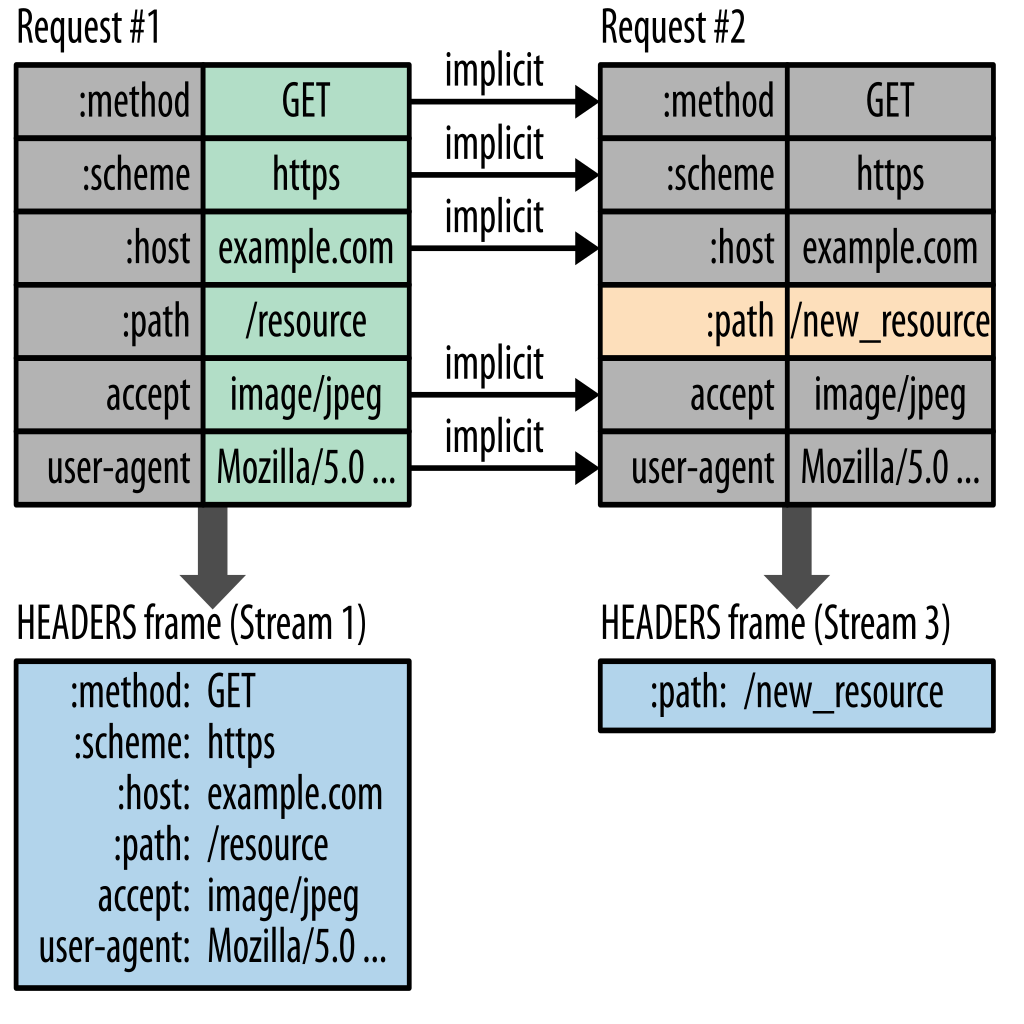
\includegraphics[width=0.6\textwidth]{hpacksavings.png}
	\caption{In HTTP/2, repeated headers are not re\hyp{}transmitted in full across requests on the same connection.}
	\label{fig:hpacksavings}
\end{figure}

Finally, HPACK also defines a static `Huffman code' which is a primitive form of compression that involves replacing characters with variable\hyp{}length sequences of bits such that the most frequent characters have shorter sequences and infrequent characters have  longer sequences~\cite{huffman}. Since the `A' character appears more frequently than the `Z' character, it gets replaced by a specific sequence of 6 bits, whereas the `Z' gets replaced by a specific sequence of 8 bits. Cloudflare, one of the first large companies to deploy HTTP/2, found that using this Huffman code alone (and even neglecting the use of the dynamic table for optimal compression) results in around 30\% header size savings compared with HTTP/1.1~\cite{huffmansavings}.
